%%RESULTADOS

\section{Adquisición de datos}
Tras realizar la evaluación del subsistema de adquisición descrito en la sección \ref{Sec: Adquisicion} utilizando el procedimiento detallado en la sección \ref{Sec: EvalAdquisicion}, se obtuvo un valor de correlación promedio de 0.915 $\pm$ 0.0604, el cual se obtuvo de un total de 40 registros realizados (3 repeticiones de cada una de las señales que conforman el banco de señales para evaluación de la adquisición). En la Figura \ref{Figura: ValProCum} se puede observar una comparación entre la señal patrón y la señal adquirida con el subsistema diseñado en Simulink\textregistered.


%Tras adquirir las señales patrón para la evaluación del bloque de adquisición descritas en la metodología, se calculó la métrica de correlación entre las señales adquiridas y las patrón, buscando traslapar una sobre otra como se muestra en la Figura \ref{Figura: ValProCum}. Al tener el valor de correlación para cada registro se obtuvo como resultado una correlación promedio de 0.9615 $\pm$ 0.0604, valor que sirve como indicador de la calidad del bloque diseñado para la adquisición y decodificación de datos.

%Senoidal obtenida tras para evaluación
\begin{figure}[htbp]
	\centering
	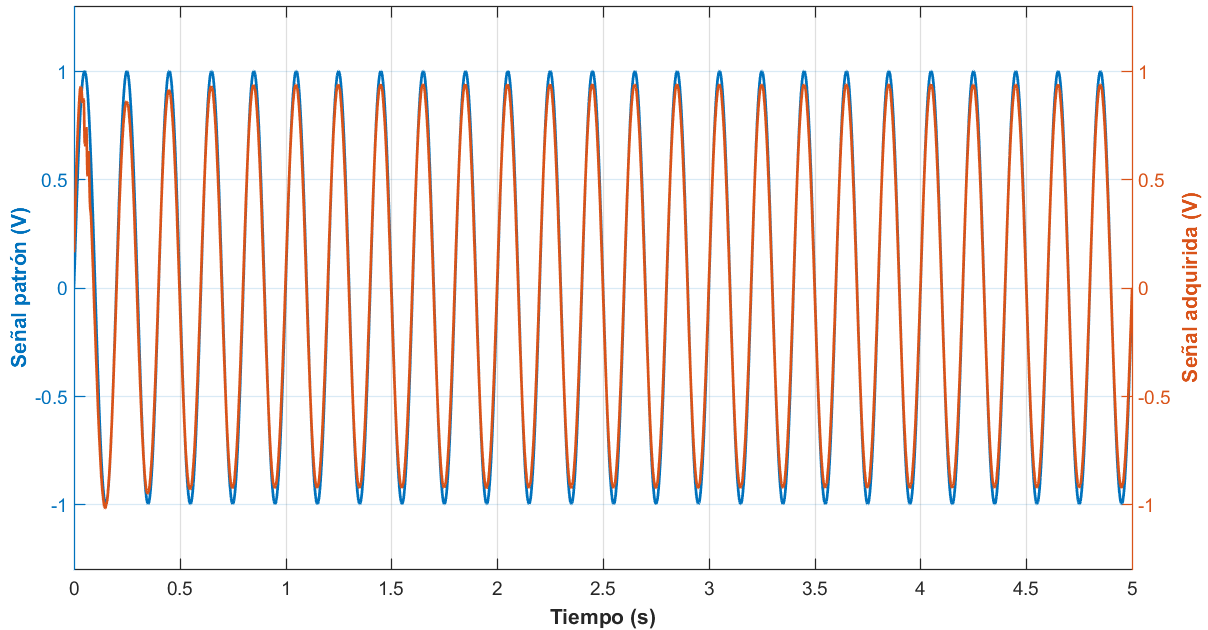
\includegraphics[width=\textwidth]{ValProCum.png}
	\caption[Comparación entre señales para evaluación de adquisición.]{Comparación entre señales para evaluación de adquisición. Señal patrón generada en MATLAB\textregistered (azul). Señal adquirida mediante el subsistema de adquisición diseñado en Simulink\textregistered (Rojo).}
	\label{Figura: ValProCum}
\end{figure}


\section{Procesamiento de sEMG}
El esquema de filtrado utilizado (filtro pasa altas, filtro pasa bajas y filtro rechaza banda), al igual que el procesamiento para obtención del RMS suavizado, se pusieron a prueba fuera de línea con 10 sujetos (6 hombres y 4 mujeres) sanos de edades entre 20 y 24 años.

La Figura \ref{Figura: Filtrado} muestra una comparación entre los canales de sEMG adquiridos para las pruebas de procesamiento y el resultado de su filtrado fuera de línea.

En la Figura \ref{Figura: RMS} se muestra un ejemplo del resultado del procesamiento para obtención de RMS suavizado.

%Utilizando los registros de calibración se probaron los filtros diseñados, obteniendo como resultado notorio la estabilización de la línea base de cada registro. En la Figura \ref{Figura: Filtrado} se muestra una comparación entre los registros crudos y filtrados de ambos canales adquiridos durante el entrenamiento.

\begin{figure}[htbp]
	\centering
	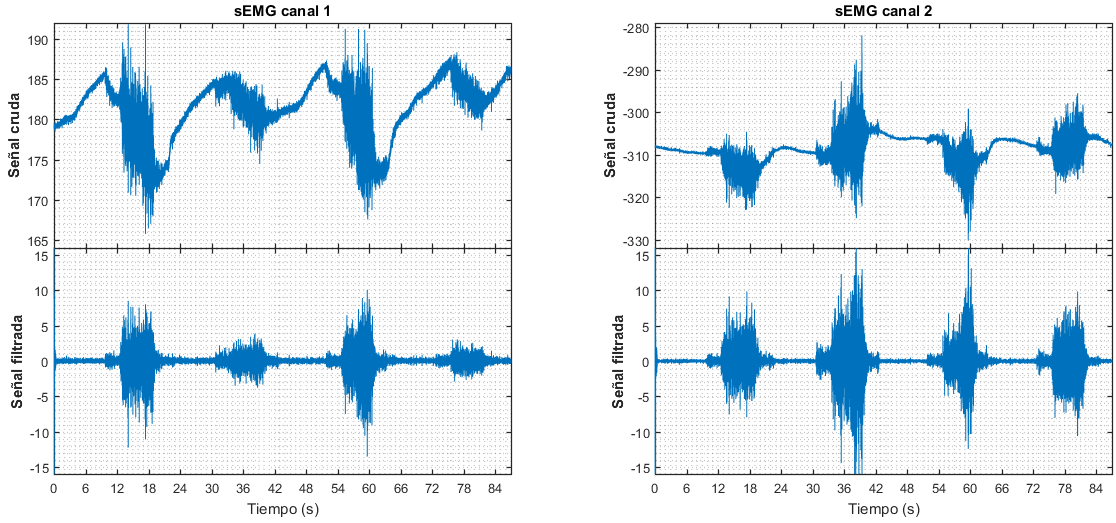
\includegraphics[width=0.8\textwidth]{Filtrado.png}
	\caption{Ejemplo representativo del funcionamiento del esquema de filtrado diseñado.}
	\label{Figura: Filtrado}
\end{figure}

%Con los registros ya filtrados se obtuvo el valor RMS a lo largo de todo el registro utilizando ventanas de 100 ms, dando como resultado una envolvente discreta de sEMG para cada canal. En la Figura \ref{Figura: RMS} se muestran los registros de sEMG filtrados con sus respectivas envolventes discretas de RMS y marcadores de la acción solicitada al sujeto durante el entrenamiento.

\begin{figure}[htbp]
	\centering
	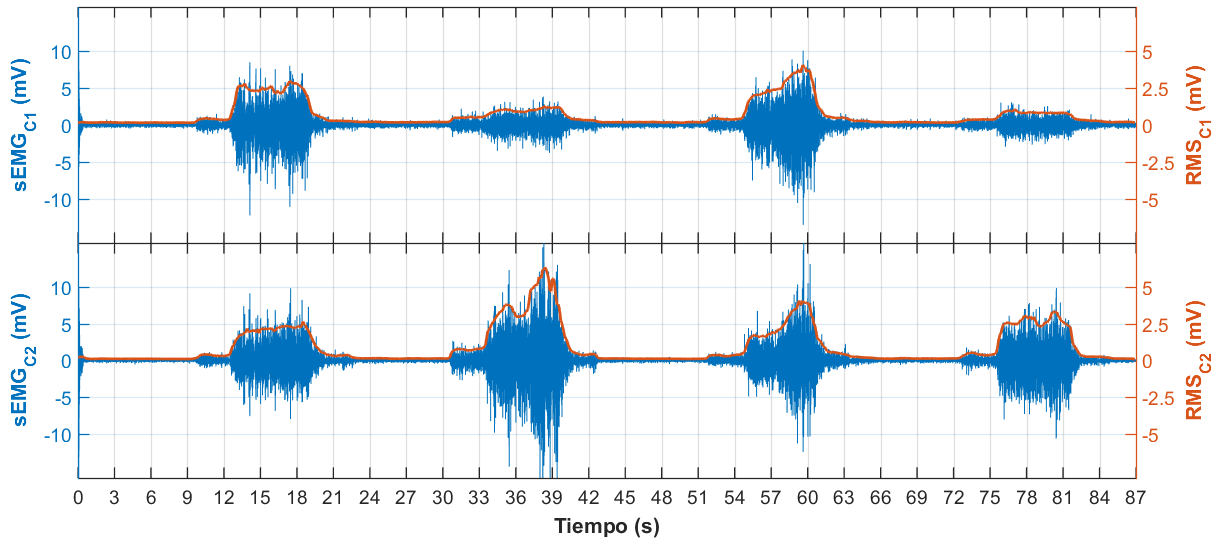
\includegraphics[width=\textwidth]{RMS.png}
	\caption[Ejemplo representativo de la obtención de envolvente de RMS]{Ejemplo representativo de la obtención de envolvente de RMS. En azul, los registros de sEMG. En rojo, las envolventes de RMS.}
	\label{Figura: RMS}
\end{figure}


\section{Sistema de control}
El sistema completo se puso a prueba con un sujeto varón sano de 22 años de edad, en el cual presentaron resultados satisfactorios. Relacionado a la validación fuera de línea, el algoritmo para la clasificación de los movimientos obtuvo un porcentaje de acierto del 81$\%$. La Figura \ref{Figura: MapOff} muestra el resultado de la prueba para la validación fuera de línea. Respecto a la prueba de validación en línea, en esta demostró una respuesta del sistema de acuerdo a lo esperado. La Figura \ref{Figura: MapOn} presenta un segmento de las señales obtenidas tras la realización de la prueba en línea. En relación a la tarea objetivo, el sistema logró llevar a cabo la modulación de la estimulación eléctrica de forma satisfactoria, con un notable retardo del sistema, el cual al medirlo como se describe en la sección \ref{Sec: TareaObj}, se obtuvo un valor de retardo de 2.3 $\pm$ 0.3553 s. La Figura \ref{Figura: Retardo} muestra un acercamiento a las señales obtenidas al termino de la tarea objetivo, donde es notorio el retardo entre la generación de la señal patrón y el inicio de la modulación de estimulación eléctrica.

Respecto a la aplicación sEMG-FES contralateral, esta se logró llevar a cabo sin complicaciones en el sujeto de prueba antes mencionado, el cual pudo realizar por completo la tarea. Las Figuras \ref{Figura: Fun_A_1} a \ref{Figura: Fun_A_2} muestran momentos en los que el sujeto llevó a cabo la tarea funcional.
%Previo a realizar pruebas del esquema de control en línea, este se probó fuera de línea, aprovechando los registros de calibración. Para estas pruebas se diseñó un script en MATLAB que obtiene los parámetros necesarios del esquema de control de la misma forma que los arroja la calibración. Una vez obtenidos dichos parámetros se configura con ellos al esquema de control y se realiza una prueba fuera de línea donde con cada ventana de sEMG se obtiene un valor de RMS el cuál es sometido al esquema de control y arroja un valor de amplitud para el canal asociado al movimiento detectado. Tras probar el esquema de control con tres registros distintos de calibración se obtuvo un porcentaje de acierto del 81$\%$ en la identificación correcta de los movimientos de cierre, apertura y descanso de mano.

%En la Figura \ref{Figura: MapOff} se muestra el resultado de  una prueba exitosa del esquema de control fuera de línea, donde se observa que el esquema de control diseñado suele presentar errores en la identificación de los segmentos iniciales y finales de la tarea apertura de mano.

\begin{figure}[htbp]
	\centering
	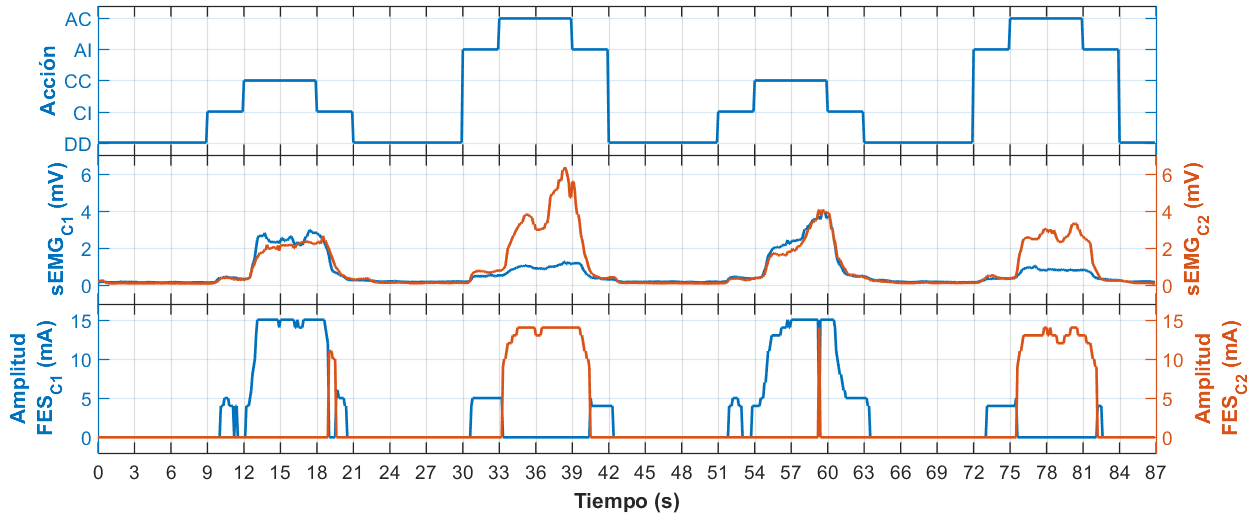
\includegraphics[width=\textwidth]{MapOff.png}
	\caption[Ejemplo representativo exitoso del funcionamiento fuera de línea del sistema de control]{Ejemplo representativo exitoso del funcionamiento fuera de línea del sistema de control. Arriba: Envolventes de sEMG (Azul: canal 1. Rojo: canal 2). Centro: Amplitudes de estimulación eléctrica (salida del sistema de control) (Azul: canal 1. Rojo: canal 2). Abajo: Marcadores de acción solicitada al sujeto (descanso (DD), pinza gruesa incompleta (CI), pinza gruesa completa (CC), apertura incompleta (AL), apertura completa (AC)).}
	\label{Figura: MapOff}
\end{figure}

%\newpage
%Para la prueba en línea se configuró el modelo de Simulink con los datos obtenidos tras la calibración, y se solicitó al sujeto realizar el seguimiento de un par de señales trapezoidales que le indicarían el tipo de movimiento que tendría que lograr. Cuando la trapezoidal estuviera en cero, tendría que mantenerse en descanso; en la pendiente positiva de la trapezoidal tendría que realizar una transición de descanso hacia el movimiento completo solicitado; en la meseta de la trapezoidal tendría que mantener el movimiento completo solicitado; y en la pendiente negativa de la trapezoidal tendría que realizar una transición del movimiento completo solicitado hacia descanso.

%En la Figura \ref{Figura: MapOn} se muestra un segmento de una de las pruebas exitosas realizadas en línea. En dicha figura se puede observar que existe un retardo entre la trapezoidal y la respuesta del sistema de control, el cual es la suma del retardo que genera el procesamiento de la señal, el retardo ocasionado por el esquema de control, y el tiempo de respuesta del sujeto a la indicación de la trapezoidal.

\begin{figure}[htbp]
	\centering
	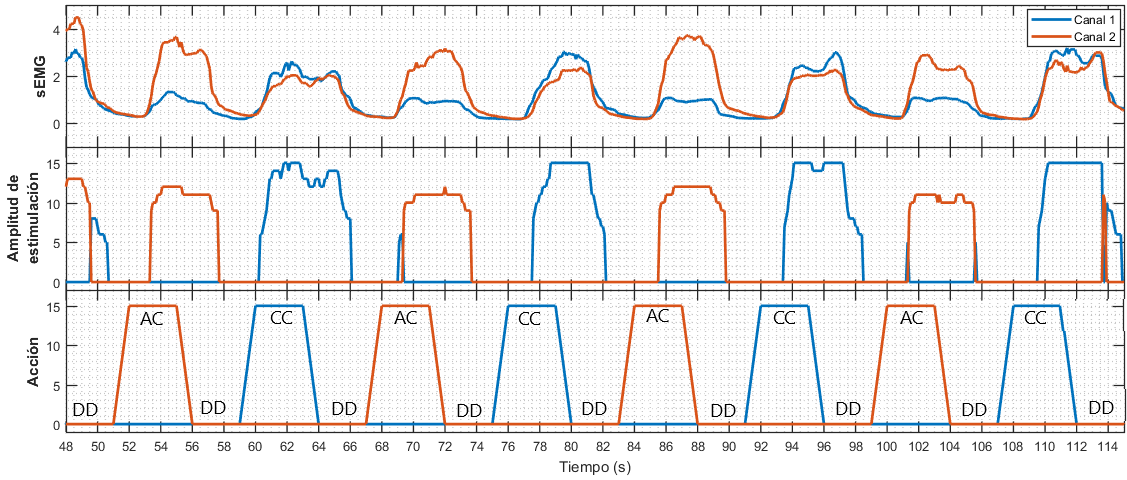
\includegraphics[width=\textwidth]{MapOn.png}
	\caption[Segmento de prueba representativa exitosa del funcionamiento en línea del sistema de control]{Segmento de prueba representativa exitosa del funcionamiento en línea del sistema de control.  Arriba: Envolventes de sEMG (Azul: canal 1. Rojo: canal 2). Centro: Amplitudes de estimulación eléctrica (salida del sistema de control) (Azul: canal 1. Rojo: canal 2). Abajo: Señal trapezoidal patrón indicadora de tarea a seguir (descanso (DD), pinza gruesa (CC), apertura completa (AC)).}
	\label{Figura: MapOn}
\end{figure}

%Para obtener el valor del retardo total se midió el tiempo existente entre el inicio de la pendiente positiva de la señal indicadora (trapezoidal) y la activación de la estimulación eléctrica. Al promediar los tiempos obtenidos a lo largo de las pruebas realizadas en línea se obtuvo un valor de 2.3 $\pm$ 0.3553 s.

%En la Figura \ref{Figura: Retardo} se muestra un acercamiento a las señales obtenidas en una prueba representativa de las pruebas realizadas en línea. Se muestran una sobre otra para visualizar el retardo existente entre el inicio de la señal indicadora y la activación de la estimulación eléctrica.

\begin{figure}[htbp]
	\centering
	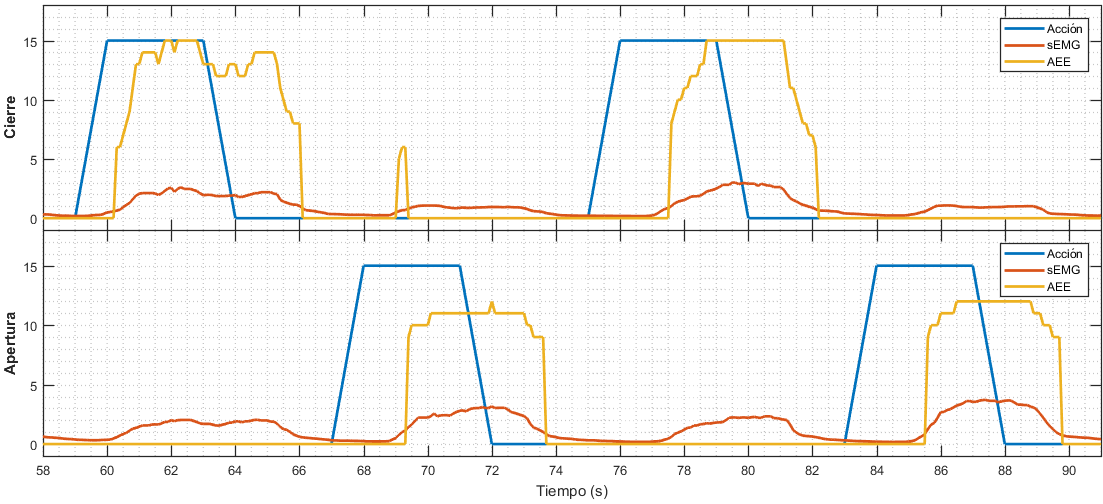
\includegraphics[width=\textwidth]{Retardo.png}
	\caption[Segmento de prueba representativa de tarea objetivo]{Segmento de prueba representativa de tarea objetivo. Se muestran las diferentes señales asociadas a cada movimiento una sobre otra para visualizar el retardo existente. Arriba: Señales para movimiento pinza gruesa completa. Abajo: Señales para movimiento apertura completa. En azul se muestra la señal trapezoidal patrón del movimiento a seguir. En rojo se muestra la envolvente de sEMG. En amarillo se muestra la amplitud de estimulación eléctrica (salida del sistema control).}
	\label{Figura: Retardo}
\end{figure}

%Posturas manos
\begin{figure}[htbp]
	\centering
	\begin{subfigure}[htbp]{0.45\textwidth}
		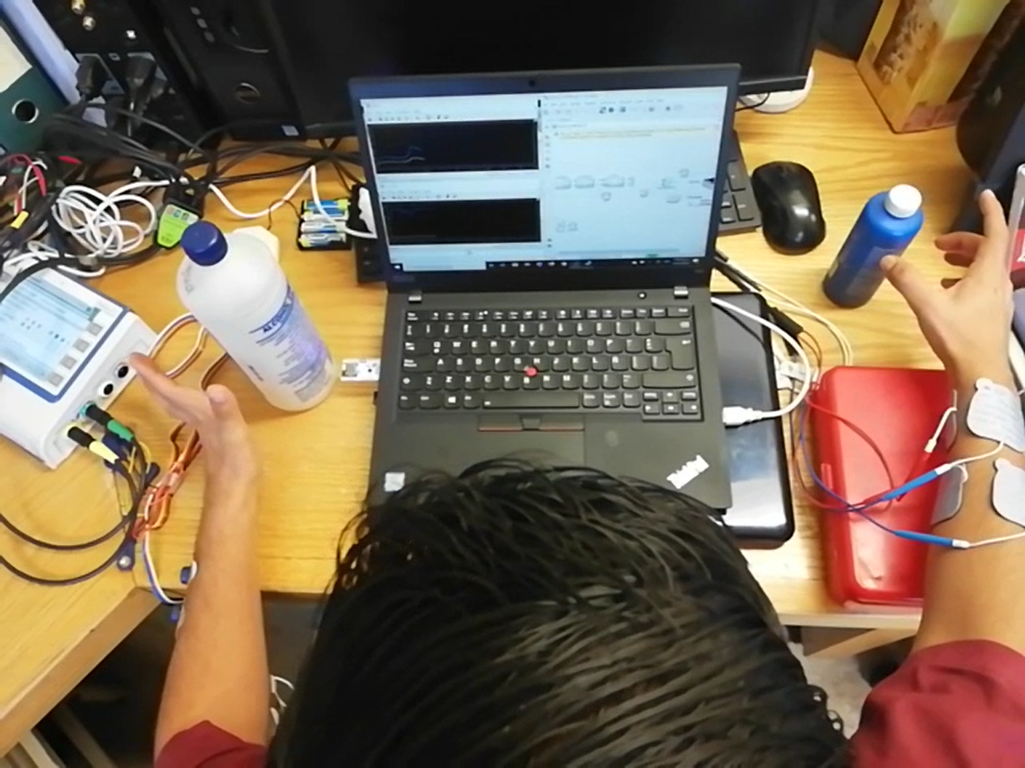
\includegraphics[width=\textwidth]{Funcional_Apertura_1.png}
		\caption{Apertura de mano para tomar objeto.}
		\label{Figura: Fun_A_1}
	\end{subfigure}
%	\hfill
	\begin{subfigure}[htbp]{0.45\textwidth}
		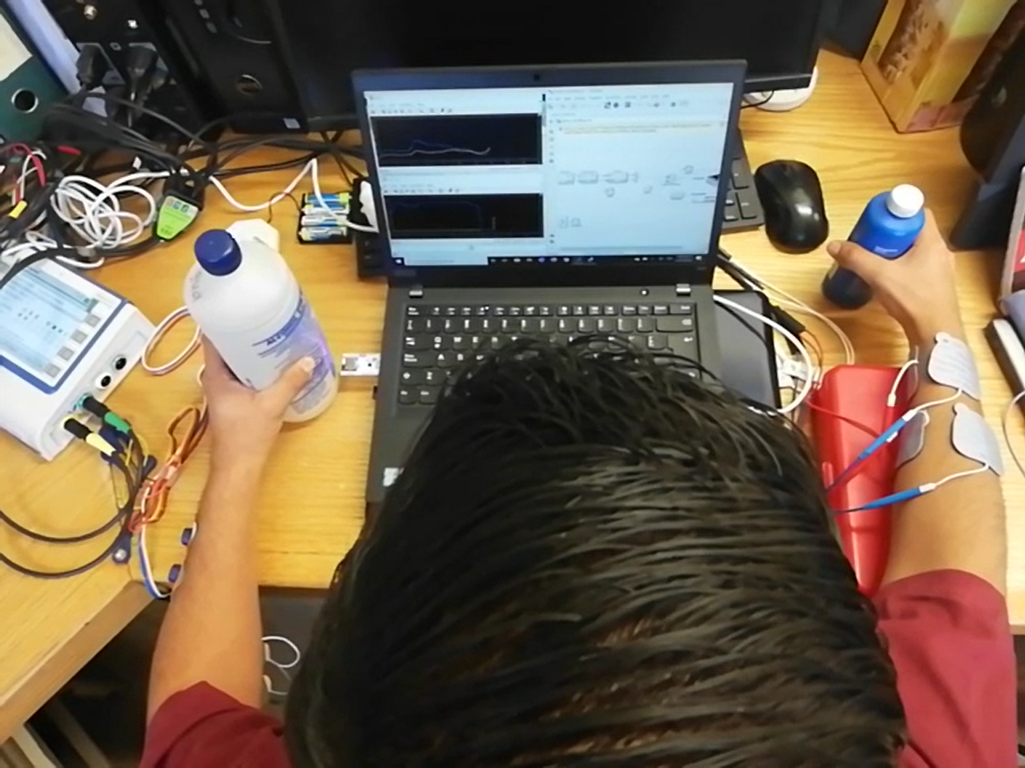
\includegraphics[width=\textwidth]{Funcional_Cierre.png}
		\caption{Pinza gruesa con objeto tomado.}
		\label{Figura: Fun_C}
	\end{subfigure}
%	\hfill
	\newline
	\begin{subfigure}[htbp]{0.45\textwidth}
		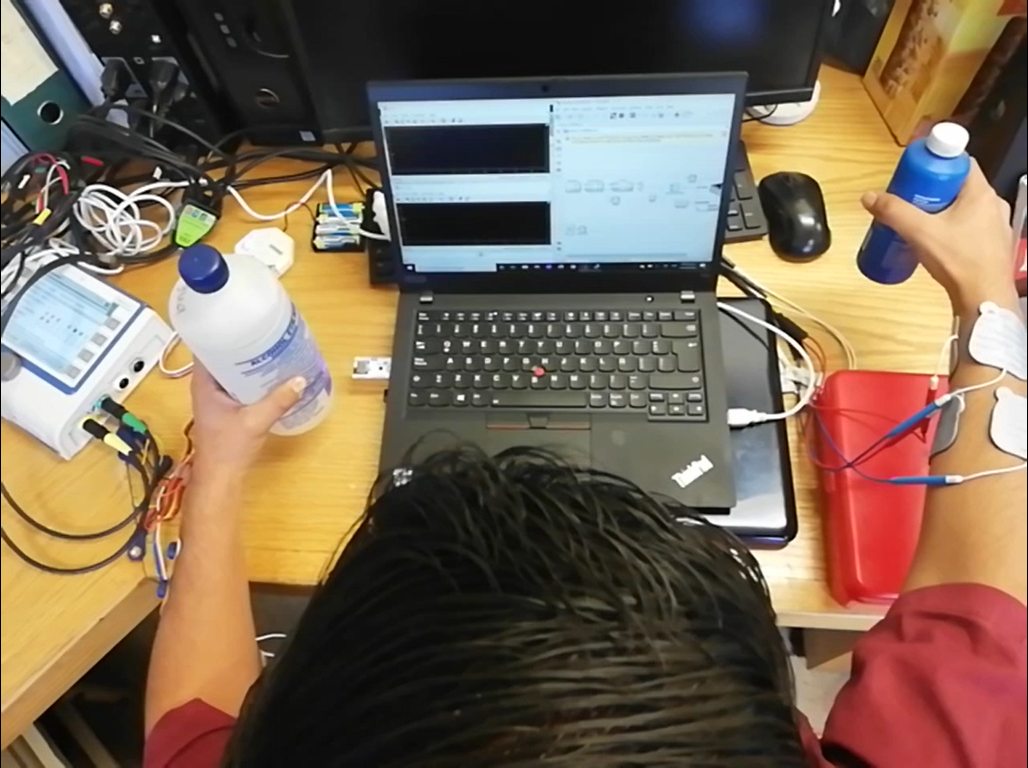
\includegraphics[width=\textwidth]{Funcional_Levantar.png}
		\caption{Levantamiento de objeto para trasladarlo.}
		\label{Figura: Fun_L}
	\end{subfigure}
%	\hfill
	\begin{subfigure}[htbp]{0.45\textwidth}
		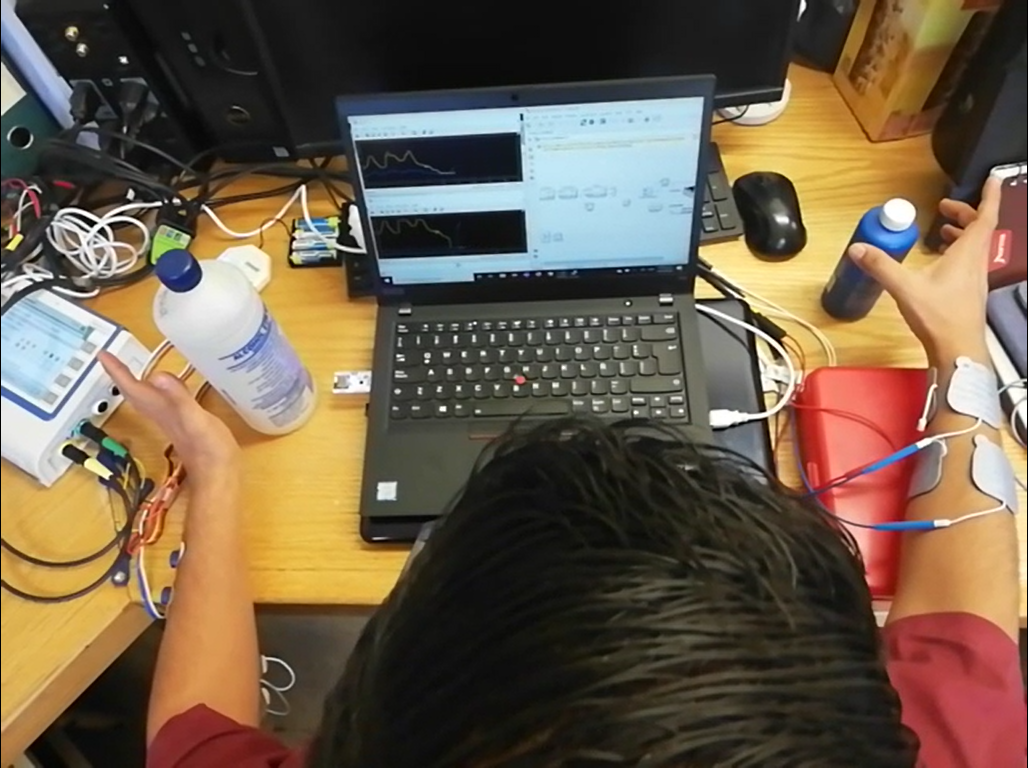
\includegraphics[width=\textwidth]{Funcional_Apertura_2.png}
		\caption{Apertura de mano para soltar objeto posterior a su traslado.}
		\label{Figura: Fun_A_2}
	\end{subfigure}
	\caption{Momentos de sujeto realizando tarea funcional.}
	\label{Figura: TareaFuncional}
\end{figure}